\documentclass{article}

\usepackage{amssymb, amsmath}
\usepackage[a4paper,top=3cm,bottom=2cm,left=2.5cm,right=2.5cm,marginparwidth=1.25cm]{geometry}
\usepackage[colorinlistoftodos]{todonotes}
\usepackage[backend=biber]{biblatex}
\addbibresource{bibliography/refs.bib}
\usepackage{mathtools}
\usepackage{stmaryrd}
\usepackage{trimclip}
\usepackage{dsfont}
\usepackage{caption}
\usepackage{graphicx}
\graphicspath{{./graphics/}}

\setlength\parindent{0pt}
\setlength\parskip{5pt}

\DeclareMathOperator{\sgn}{sgn}
\DeclareMathOperator{\tr}{Tr}
\DeclareMathOperator{\vect}{vec}
\DeclareMathOperator{\tri}{tridiag}



\newlength{\nnearrowheight}
\newlength{\ssearrowheight}
\settoheight{\nnearrowheight}{$\nnearrow$}
\settoheight{\ssearrowheight}{$\ssearrow$}
\newcommand{\bQ}{\mathds{Q}}
\newcommand{\bR}{\mathds{R}}
\newcommand{\bN}{\mathds{N}}
\newcommand{\bZ}{\mathds{Z}}
\newcommand{\bC}{\mathds{C}}
\newcommand{\bottomofnnearrow}{\makebox{\clipbox{0pt 0pt 0pt {.5\totalheight}}{$\nnearrow$}}}
\newcommand{\topofnnearrow}{\raisebox{.37\nnearrowheight}[.5\nnearrowheight][0pt]{\makebox{\clipbox{0pt {.5\totalheight} 0pt 0pt}{$\nnearrow$}}}}
\newcommand{\bottomofssearrow}{\makebox{\clipbox{0pt 0pt 0pt {.5\totalheight}}{$\ssearrow$}}}
\newcommand{\topofssearrow}{\raisebox{.37\ssearrowheight}[.5\ssearrowheight][0pt]{\makebox{\clipbox{0pt {.5\totalheight} 0pt 0pt}{$\ssearrow$}}}}
\newcommand{\upweakto}{\mathrel{%
    %\bottomofnnearrow%
    \hspace*{-.3pt}\makebox[0pt]{$-$}\hspace*{.35pt}%
    \topofnnearrow\hspace*{-.65pt}%
}}
\newcommand{\downweakto}{\mathrel{%
    %\hspace*{-.65pt}\topofssearrow%
    \hspace*{-.7pt}\makebox[0pt]{$-$}\hspace*{.35pt}%
    \bottomofssearrow%
}}

\DeclarePairedDelimiter\abs{\lvert}{\rvert}%
\DeclarePairedDelimiter\norm{\lVert}{\rVert}%

\makeatletter
\let\oldabs\abs
\def\abs{\@ifstar{\oldabs}{\oldabs*}}
%
\let\oldnorm\norm
\def\norm{\@ifstar{\oldnorm}{\oldnorm*}}
\makeatother

\newtheorem{theorem}{Theorem}[section]
\newtheorem{corollary}{Corollary}[theorem]
\newtheorem{lemma}[theorem]{Lemma}
\newtheorem{definition}{Definition}[section]


\author{Farid Kaveh}
\title{The Hermitian Splitting Method for Positive Definite Systems}


\begin{document}
  \begin{center}
      \large\textbf{THE HERMITIAN SPLITTING METHOD FOR POSITIVE DEFINITE SYSTEMS \\}
      \small\textbf{A REVIEW AND SUMMARY\\}
      \vspace{5pt}
      FARID KAVEH
  \end{center}


\section{HSS and IHSS Iteration: Key Results}
In a 2003 paper \cite{bai2003hermitian}, Bai and Golub introduced a new iterative method for solving large sparse systems of the form

\begin{equation}\label{main_system}
    Ax = b, \; \; A \in \bC^{n \times n}, \; x,b \in {\bC^n},
\end{equation}

where $A$ is non-singular, in general non-Hermitian, and positive definite. They called this method the Hermitian/skew-Hermitian splitting iteration (HSS), and provided also an inexact Hermitian/skew-Hermitian splitting iteration (IHSS) method which is more efficient in solving large systems. Note that a non-Hermitian matrix $A$ is said to be positive definite if its Hermitian part $H = \frac{1}{2}(A + A^\ast)$ is positive definite.

Here we shall analyse the ideas behind the HSS and IHSS techniques, as well as provide some numerical results that demonstrate the theory. We will discuss some methods for optimal parameter estimation and selection that have thus far been presented in the literature, and we will also introduce a new method of optimal parameter estimation. We will state some key results without reproducing the proofs. The exact solution of Equation \ref{main_system} shall be denoted by $x^\ast \in \bC^n$ throughout. We will need to consider \textit{splittings} of $A$. These are decompositions of the form $A = M - N$ where $M$ is a non-singular matrix.

\subsection{Statements and Explanations}
Lemma \ref{general_splittings_method} is the main lemma of \cite{bai2003hermitian}.

\begin{lemma}\label{general_splittings_method}
    Let $A \in \bC^{n \times n}, \; A = M_i - N_i \: (i = 1,2)$ be two splittings of the matrix $A$, and let $x^{(0)}\in \bC^n$ be a given initial vector. If $\{ x^{(k)}\}$ is a two-step iteration sequence defined by

    $$ \begin{Bmatrix} M_1x^{(k+\frac{1}{2})} = N_1x^{(k)}+b, \\
         M_2x^{(k+1)} = N_2x^{(k+ \frac{1}{2})}+b,\end{matrix}$$


$k = 0,1,2, \ldots$, then

$$x^{(k+1)} = M_2^{-1}N_2M_1^{-1}N_1x^{(k)} + M_2^{-1}(I + N_2M_1^{-1})b, \;\;k =   0,1,2,\ldots\;.$$
Moreover, if the spectral radius $\varrho(M_2^{-1}N_2M_1^{-1}N_1)$ of the iteration matrix $M_2^{-1}N_2M_1^{-1}N_1$ is less than $1$, then the iterative sequence $\{ x^{(k)} \}$ converges to $x^\ast$ for all initial vectors $x^{(0)} \in \bC^n$.
\end{lemma}

Letting $T: \bC^n \rightarrow \bC^n$ be the mapping given by $T(x) = M_2^{-1}N_2M_1^{-1}N_1x + M_2^{-1}(I + N_2M_1^{-1})b$, $T$ will be a contraction mapping whenever
\begin{align}\label{contraction_condition}
    \norm{T(x) - T(y)}_2 = \norm{ M_2^{-1}N_2M_1^{-1}N_1(x-y)}_2 \leq \norm{x-y}_2, \; \; \text{for all}\: x,y \in \bC^n
\end{align}

Moreover, $x^\ast$ is a fixed point of $T$. It is easy to see that Inequality \ref{contraction_condition} will be satisfied when the spectral norm of the iteration matrix\footnote{The requirement of the lemma is that the spectral \textit{radius} of the iteration matrix be less than 1, and the spectral radius is less than or equal to the spectral norm in general. Although, in the case of the HSS iteration, the iteration matrix is Hermitian, so the spectral radius and the spectral norm coincide.} is less than $1$. In this case the Banach fixed-point theorem guarantees convergence of the iteration to the unique fixed point $x^\ast \in \bC^n$. The HSS method exploits the fact that if $A$ is a positive definite matrix, then $T$ is necessarily a contraction for a class of pairs of splittings $A = M_i - N_i, \: i=1,2$, described below.

Let $H = \frac{1}{2}(A + A^\ast)$, $S = \frac{1}{2}(A - A^\ast)$ be the Hermitian and skew-Hermitian parts of $A$, respectively. Then the HSS iteration method is defined by taking the two splittings $A = (H + \alpha I) - (\alpha I - S)$, $A = (\alpha I + S ) - (\alpha I - H)$ for $\alpha > 0$ and then proceeding as in Lemma \ref{general_splittings_method}. More formally, the HSS method can be defined as below.

\hspace{2mm} \textbf{The HSS iteration method.} \textit{Given an initial guess $x^{(0)}$, for $k = 0,1,2,\ldots$, until $\{ x^{(k)}\}$ converges compute}

$$
    \begin{Bmatrix} (\alpha I + H)x^{(k+\frac{1}{2})} = (\alpha I - S)x^{(k)} +b, \\
    (\alpha I + S)x^{(k+1)} = (\alpha I - H)x^{(k +\frac{1}{2})} + b,\end{matrix}
$$

\textit{where $\alpha$ is a given positive constant.}

It is readily seen that the iteration matrix for the HSS methods is given by
\begin{equation}
    \mathcal{M}(\alpha) = (\alpha I + S )^{-1}(\alpha I - H)(\alpha I + H)^{-1}(\alpha I -S).
\end{equation}

Crucially, Bai and Golub obtained an upper bound \cite{bai2003hermitian} for the spectral radius of $\mathcal{M}(\alpha)$,  $\varrho(\mathcal{M}(\alpha)) \leq \sigma(\alpha)$, given by

\begin{equation}
    \sigma(\alpha )\equiv \max_{\lambda_i \in \lambda(H)}\abs{\frac{\alpha - \lambda_i}{\alpha + \lambda_i}},
\end{equation}
where $\lambda(H)$ is the spectrum of $H$. Now if $A$ is positive definite, then so is $H$, hence $\lambda_i > 0, \; i = 1, 2, \ldots, n$. In such a case we will have
\begin{equation}\label{convergence_of_HSS}
    \varrho(\mathcal{M}(\alpha)) \leq \sigma(\alpha) < 1,
\end{equation}

and so the HSS iteration will converge to $x^\ast$ for positive definite $A$. Moreover, the upper bound $\varrho(\mathcal{M}(\alpha)) \leq \sigma(\alpha)$ is independent of the spectrum of $A$ or $S$. Indeed, if $\gamma_{R},\gamma_{r} >0$ are the maximum and minimum eigenvalues of $H$ respectively,  then the optimal value of $\alpha$ is given by \cite{bai2003hermitian} $\bar{\alpha} = \sqrt{\gamma_R \gamma_r}$, and consequently

\begin{equation}\label{spectral_condition}
    \sigma(\bar{\alpha}) = \frac{\sqrt{\gamma_{R}} -\sqrt{\gamma_r}}{\sqrt{\gamma_{R}}+\sqrt{\gamma_{r}}} = \frac{\sqrt{\kappa(H)} - 1}{\sqrt{\kappa(H)} + 1}.
\end{equation}
Here $\kappa(H)$ is the spectral condition number of $H$.\footnote{The spectral condition number is defined only for diagonalizable matrices. It is a measure of the sensitivity of the eigenvalues of a diagonalizable matrix to small perturbations. For a definition of the spectral condition number see \cite{JIANG1997165}} Notice that $\bar{\alpha}$ minimises $\sigma(\alpha)$ but not necessarily $\varrho(\mathcal{M}(\alpha))$.

Since exact solution to the inner systems of the HSS iteration method can be costly to obtain, the inexact HSS iteration, or IHSS iteration, may be more useful in practice when solving large systems. This method is analogous to the HSS iteration except that the inner systems are now solved via approximate methods. It is stated in \cite{bai2003hermitian} as follows.

\textbf{The IHSS iteration method} \textit{Given an initial guess $\bar{x}^{(0)}$, for $k = 0,1,2,\ldots$, until $\{ x^{(k)}\}$ converges,  }

1. \textit{approximate the solution of $(\alpha I + H)\bar{z}^{(k)} = \bar{r}^{(k)} \; (\bar{r}^{(k)} = b - A\bar{x}^{(k)})$ by iterating the residue satisfies}


$$ \frac{\norm{\bar{r}^{(k)} - (\alpha I + H)\bar{z}^{(k)}}}{\norm{\bar{r}^{(k)}}} \leq \epsilon_k ,$$

\textit{and then compute $\bar{x}^{(k+\frac{1}{2})} = \bar{x}^{(k)} + \bar{z}^{(k)};$} \newline
2. \textit{approximate the solution of $(\alpha I + S)\bar{z}^{(k+\frac{1}{2})} = \bar{r}^{(k+\frac{1}{2})} \; (\bar{r}^{(k+\frac{1}{2})} = b - A\bar{x}^{(k+\frac{1}{2})})$ by iterating until $\bar{z}^{(k+\frac{1}{2})}$ is such that the residual satisfies}

$$\frac{\norm{\bar{r}^{(k+\frac{1}{2})} - (\alpha I + S)\bar{z}^{(k+\frac{1}{2})}}}{\norm{\bar{r}^{(k+\frac{1}{2})}}} \leq \eta_k,$$
\textit{and then compute $\bar{x}^{(k+1)} = \bar{x}^{(k+\frac{1}{2})} + \bar{z}^{(k+\frac{1}{2})}.$}

The convergence analysis for the IHSS iteration is more complicated than that of the exact HSS iteration, since convergence now depends not only on the spectral condition number of $H$, but also on the relative errors $\{ \epsilon_k \}$ and $\{ \eta_k \}$ of the inner system solutions. The following is the main result of Bai and Golub \cite{bai2003hermitian} regarding the convergence of the IHSS iteration.

\begin{theorem}
    Let $\{ \bar{x}^{(k)}\}$ be the sequence generated by the IHSS iteration given some initial guess $\bar{x}^{(0)}$. Then let
    $$\varrho = \norm{(\alpha I + S)(\alpha I + H)^{-1}}_2, \; \; \theta = \norm{A(\alpha I + S)^{-1}}_2,$$

    and also $\eta_R = \max{ \{ \eta_k \} }$, $\epsilon_R = \max{ \{ \epsilon_k\}}$. If $(\sigma(\alpha) + \theta \varrho \eta_R)(1 + \theta \epsilon_R) < 1$, then $\{\bar{x}^{(k)}\}$ converges to $x^\ast$.
\end{theorem}

Note that convergence does not require the limit of $\epsilon_k$ for large $k$ to approach zero. Likewise for the limit of $\eta_k$.

In terms of computational complexity, the cost of the $k$-th IHSS iteration is $\mathcal{O}(4n + 2a + \chi_k(H)+\chi_k(S))$, where $a$ is the cost of computing $Ay$ for some $y\in \bC^n$,\footnote{this may be $o(n^2)$ if $A$ has sparse structure} and $\chi_k(H)$ and $\chi_k(S)$ are the costs of solving the first and second inner systems, respectively, on the $k$-th iteration.
\subsection{Discussion}

The HSS and IHSS iteration methods have the great benefit that the convergence of the generated sequence can be controlled through the conditioning of $H$, instead of the condition number of $A$. This is evident from Equation \ref{spectral_condition}, where the convergence rate of the HSS method is bounded above by considering only the condition number of $H$ and not that of $S$.  However, even the optimal $\sigma(\bar{\alpha})$ is in many cases a very generous upper bound for $\varrho(\mathcal{M}(\alpha))$, meaning that our control over the convergence through the condition number of $H$ is weak.\footnote{see for example Bai and Golub's numerical experiments in applying the HSS iteration to the problem of the convection-diffusion equation in the unit cube \cite{bai2003hermitian}}

Moreover, the HSS and IHSS methods are limited by the efficiency of the solvers used to resolve the inner systems. Hence, more analysis is required to understand the structure of the inner systems for a given application, and to select appropriate solvers accordingly.


\section{Optimal Parameter Selection}

Of great interest to the application of HSS iteration and related methods is the optimal selection of the parameter $\alpha$. As discussed in the foregoing section, while $\bar{\alpha}$ minimises the upper bound for the convergence rate of the iteration, it does not in fact minimise the convergence rate itself. Great effort has been made in finding a prescriptive method of determining $\alpha^\ast = \arg \min_\alpha \{ \varrho(\mathcal{M}(\alpha))\}$. In \cite{two_two_block_optimal} Bai and collaborators consider the problem for two-by-two block matrices with some success. In \cite{HUANG2014142}, Huang considers the problem more generally and obtains a cubic polynomial in terms of the traces of some matrices. A positive real solution to this cubic then gives an estimate of $\alpha^\ast$.

\subsection{Optimal Parameter Selection for Two-by-Two Matrices}
Suppose the matrix $A$ in Equation \ref{main_system} is of the form

\begin{equation}\label{two_two_block}
    A = \begin{pmatrix} \lambda_1 I_r && E \\
-E^\ast && \lambda_2 I_s \end{pmatrix}, \; \; \lambda_1 \geq \lambda_2 > 0
\end{equation}

 where $I_r \in \bC^{r \times r}, \; I_s \in \bC^{s \times s}$ are the identities in their respective spaces, and $E \in \bC^{r \times s}$. In \cite{two_two_block_optimal} the authors seek $\alpha^\ast$ for the class of matrices in (\ref{two_two_block}). In doing so they first consider the general case for real two-by-two matrices. Let $A \in \bR^{2\times 2}$ and $H = \frac{1}{2}(A + A^\ast)$ with eigenvalues $\lambda_1 \geq \lambda_2 > 0$, and $ S = \frac{1}{2}(A - A^\ast)$ has determinant $\det(S) = q^2, \: q \in \bR$. Then it is found that the eigenvalues of $\mathcal{\alpha}$ are given by

\begin{equation}
    \lambda_{\pm} = \frac{(\alpha^2- \lambda_1\lambda_2)(\alpha^2-q^2)\pm\sqrt{(\alpha^2-\lambda_1\lambda_2)^2(\alpha^2-q^2)^2 - (\alpha^2-\lambda_1^2)(\alpha^2-\lambda_2^2)(\alpha^2+q^2)^2}}{(\alpha+\lambda_1)(\alpha+\lambda_2)(\alpha^2+q^2)}
\end{equation}

and so if

\begin{equation}\label{first_condition}
    (\alpha^2 - \lambda_1\lambda_2)^2(\alpha^2- q^2) \geq (\alpha^2 - \lambda_1^2)(\alpha^2 - \lambda_2^2)(\alpha^2 + q^2)^2
\end{equation}
then $\varrho({\mathcal{M}(\alpha)})$ is given by
\begin{equation}
    \label{first_varrho}
    \frac{\abs{\alpha^2- \lambda_1\lambda_2}\abs{\alpha^2-q^2}+\sqrt{(\alpha^2-\lambda_1\lambda_2)^2(\alpha^2-q^2)^2 - (\alpha^2-\lambda_1^2)(\alpha^2-\lambda_2^2)(\alpha^2+q^2)^2}}{(\alpha+\lambda_1)(\alpha+\lambda_2)(\alpha^2+q^2)}.
\end{equation}

Otherwise if

\begin{equation}\label{second_condition}
    (\alpha^2 - \lambda_1\lambda_2)^2(\alpha^2-q^2)^2 < (\alpha^2 - \lambda_1^2)(\alpha^2 - \lambda_2^2)(\alpha^2 + q^2)^2
\end{equation}

then $\varrho(\mathcal{M}(\alpha))$ is equal to

\begin{equation}\label{second_varrho}
    \sqrt{\frac{(\alpha - \lambda_1)(\alpha - \lambda_2)}{(\alpha + \lambda_1)(\alpha + \lambda_2)}}.
\end{equation}

Minimising $\varrho(\mathcal{M}(\alpha))$ by simply differentiating the above expressions and solving for local minima is not straightforward due to the square root term in (\ref{first_varrho}). However, it is possible through some analysis to derive the result stated in Lemma \ref{optimal_two_two_lemma}.

\begin{lemma}\label{optimal_two_two_lemma}
    Let $A \in \bR^{2\times2}$. Let also $H = \frac{1}{2}(A + A^T)$ have eigenvalues $\lambda_1 \geq \lambda_2 > 0$ and $S = \frac{1}{2}(A - A^T)$ have $\det(S) = q^2, \: q\in \bR$. Define also the polynomials
\begin{align*}
p_1(x) &= (x^2 + q^2)^2(x^2 - \lambda_1^2)(x^2-\lambda_2^2) - (x^2-q^2)^2(x^2-\lambda_1\lambda_2), \\
p_2(x)  &= (x^2 + q^2)^2(\lambda_1^2 - x^2)(x^2-\lambda_2^2) - (x^2-q^2)^2(x^2-\lambda_1\lambda_2).
\end{align*}

Then $\alpha^\ast = \arg \min_{\alpha} \{\varrho(\mathcal{M}(\alpha))\} $ is contained in the finite set

\begin{equation}
    S = \{ \alpha > 0: p_1(\alpha) = 0 \; \: \text{or} \; \: p_2(\alpha) = 0 \}
\end{equation}
\end{lemma}

The key insight in the proof of Lemma \ref{optimal_two_two_lemma} is that $\varrho(\mathcal{M}(\alpha))$ is minimised when $\lambda_{\pm}$ have the same modulus. Then one derives a sufficient condition for this, in this case that one of $p_1(\alpha) = 0$ or $p_2(\alpha) = 0$ is satisfied. If some additional conditions are met, this result can be extended to matrices of the form introduced in (\ref{two_two_block}). The idea of the proof in this case is to decompose $A$ into a direct sum of real two-by-two matrices and then proceed as in the proof of Lemma \ref{optimal_two_two_lemma} (although the details are much more involved).

\begin{theorem}
    With $A$ as in (\ref{two_two_block}) and with the non-zero singular values of $E \in \bC^{r \times s}$  satisfying $q_1 \geq q_2 \geq \ldots \geq q_k$. Then if $\lambda_1 = \lambda_2 = \lambda^\ast$, we will have $\alpha^\ast = \lambda^\ast$. Otherwise if $\lambda_1 > \lambda_2 > 0$, then  $\alpha^\ast$ is either a solution to

    $$(x - \sqrt{\lambda_1\lambda_2})(x - \sqrt{q_1q_2}) = 0,$$

    or it is a root of one of the following polynomials.

    \begin{align*}
        p_1^j(x) &= (x^2 + q_j^2)^2(x^2 - \lambda_1^2)(x^2-\lambda_2^2) - (x^2-q_j^2)^2(x^2-\lambda_1\lambda_2), \; \; j \in \{1,k\},\\
        p_2^j(x) &= (x^2 + q_j^2)^2(\lambda_1^2-x^2)(x^2-\lambda_2^2) - (x^2-q_j^2)^2(x^2-\lambda_1\lambda_2), \; \; j \in \{1, k\}.
    \end{align*}
\end{theorem}

\subsection{A Very General Estimate}

Another approach (taken in \cite{HUANG2014142}) is to recast the HSS iteration method as a single-step iteration and consider the behaviour of this mathematically equivalent formulation. Returning now to the general case of (\ref{main_system}), If we define

\begin{equation}\label{N_alpha_introduce}
    M(\alpha) \coloneqq \frac{1}{2\alpha}(\alpha I + H)(\alpha I + S), \; \; N(\alpha) \coloneqq \frac{1}{2\alpha}(\alpha I - H)(\alpha I - S)
\end{equation}

This gives a splitting $A = M(\alpha) - N(\alpha)$. This splitting then generates a single-step iteration process defined by the recursive relationship

\begin{equation}
    M(\alpha)x^{(k+1)} = N(\alpha) x^{(k)} + b, \; \; k = 0, 1, 2, \ldots \: .
\end{equation}

Indeed, this iterative process converges to $x^\ast$ if the spectral radius of the iteration matrix $M(\alpha)^{-1}N(\alpha)$ is less than 1. Now, since $H$ is positive definite, $(\alpha I + H)$ is never singular for $\alpha >0$, so we can formally write

\begin{equation}
    (\alpha I + H )^{-1} = \sum_{k = 0}^\infty (-1)^{k}\alpha^{-k}H^k.
\end{equation}

This implies that the commutator $[H, (\alpha I + H )^{-1} ] = 0$ and so

\begin{align*}
    M(\alpha)^{-1}N(\alpha) &= (\alpha I + S)^{-1}(\alpha I + H)^{-1}(\alpha I - H)(\alpha I - S) \\
     &= (\alpha I + S)^{-1}(\alpha I - H)(\alpha I + H)^{-1}(\alpha I - S) = \mathcal{M}(\alpha).
\end{align*}

Hence, to minimise $\varrho(\mathcal{M}(\alpha))$ we may consider minimising $N(\alpha)$ so that $M(\alpha)^{-1}N(\alpha) \approx 0$. This may be done by considering the minimum of the function

\begin{equation}
    \Phi(\alpha) \coloneqq \norm{N(\alpha)}_F^2 = \tr(N(\alpha)N(\alpha)^\ast),
\end{equation}

where $\norm{\cdot}_F$ is the Frobenius norm. Through straightforward calculation, minimising $\Phi(\alpha)$ turns out to be equivalent to minimising the polynomial \cite{HUANG2014142}\footnote{It does seem that in \cite{HUANG2014142} the minimised quantity is $4\alpha^2\Phi(\alpha)$. Based on numerical experiments, this appears to be more than good enough for applications, however it is an estimate of the optimal parameter and not an exact figure.}

\begin{equation}\label{to_minimise}
    \phi(\alpha) \coloneqq 4n\alpha^3 + 3a\alpha^2 + 2b\alpha + c.
\end{equation}

with

\begin{equation}
a = -2\tr(H), \; \; b = \tr(H^2)-\tr(S^2), \; \; c = 2\tr(HS^2), \; \; d= -\tr(H^2S^2).
\end{equation}

Since in the HSS iteration method we have $\alpha > 0$, of interest are positive real roots of $\phi(\alpha)$. It is also a fact that for $V \in \bC^{n\times n}$ Hermitian positive definite and $U \in \bC^{n\times n}$ skew-Hermitian, $\tr(VU^2) \leq 0$ \cite{HUANG2014142}, in particular we have $c \leq 0$. Clearly if $c < 0$  we will have a positive real root of $\phi(\alpha)$. Otherwise if $c = 0$ then $\alpha = 0$ is one root and the other two roots are

$$ \alpha_{\pm} = \frac{-3a \pm \sqrt{9a^2 - 32nb}}{8n},$$

so we will have a positive real solution whenever  $9a^2 - 32nb \geq 0$. If in any case there is more than one positive root of $\phi(\alpha)$, then we will have to check which is the global minimiser of $\Phi(\alpha)$.

Numerical experiments show that this method outperforms that purposed in \cite{two_two_block_optimal} in required CPU times and iteration count, even when the system is of the type seen in (\ref{two_two_block}).\cite{HUANG2014142}

\subsection{A New Method of Estimation}

The estimation method for the selection of $\alpha$ discussed in the previous subsection has the advantage that it is quite general and makes very few assumption about the structure of $A$. However, in some cases, such as when using finite difference methods to solve the convection-diffusion equation, we do in fact know a lot about the sparsity structure of $A$. In particular, using the scheme discussed in Section 3, we will have for the convection-diffusion problem that

\begin{equation}\label{herm}
    H = H_x \otimes I \otimes I + I \otimes H_y \otimes I + I \otimes I \otimes H_z,
\end{equation}

where we have defined

\begin{equation}
    H_x = \tri(1, 6, -1), \; \; H_y = H_z = \tri(1,0,-1).
\end{equation}

We will also have the skew-Hermitian part

\begin{equation}\label{skew_herm}
    S = S_x \otimes I \otimes I + I \otimes S_y \otimes I + I \otimes I \otimes S_z,
\end{equation}

where

\begin{equation}
    S_\xi = \tri(-r_\xi, 0 , r_\xi), \; \; \xi \in \{x,y,z \},
\end{equation}

with the $r_\xi$ known parameters of the problem. For this class of problem we introduce a new method of estimating the optimal value of $\alpha$. The idea is again to minimise $N(\alpha)$ introduced in (\ref{N_alpha_introduce}) for some choice of metric, but instead of minimising the Frobenius norm $\norm{N(\alpha)}_F$ we will instead minimise an upper bound on the spectral norm
\begin{equation}
    \Psi(\alpha) \coloneqq \norm{N(\alpha)}_2.
\end{equation}
 In the interest of brevity we will consider the case where $r_\xi = r$ for all $ \xi \in \{x,y,z\}$, but the method can be immediately extended to the more general case. We will also have need of the following bound, sometimes called `Schur's test'.\cite{MATHIAS1990269}

For any $A \in \bC^{m\times n}$,

\begin{equation}
    \norm{A}_2 = \sqrt{\norm{A}_\infty\norm{A}_1}.
\end{equation}

Moreover, since $\norm{\cdot}_2$ is induced by the 2-norm on $\bC^n$ it is submultiplicative. Note first of all that given the structure of $H$ and $S$, we have

\begin{align}
    \norm{\alpha I - H}_\infty &= \norm{\alpha I - H}_1 = (\abs{6- \alpha} + 4)\\
    \norm{\alpha I - S}_\infty &= \norm{\alpha I - S}_1 = (\alpha + 4r).
\end{align}

These together give

\begin{align}
    \Psi(\alpha) &= \frac{1}{2\alpha}\norm{(\alpha I - H)(\alpha I - S)} \nonumber \\
    &\leq \frac{1}{2\alpha}\norm{\alpha I -H}_2 \norm{\alpha I - S}_2 \nonumber\\
    &\leq \frac{1}{2\alpha}\norm{\alpha I -H}_1 \norm{\alpha I - S}_1 \nonumber\\
    &= \frac{1}{2\alpha}(\alpha + 6r)(\abs{6- \alpha} + 6)
\end{align}
From Figure \ref{optimal_alpha_fig} it is clear that $\alpha = 6$ is the value that always minimises this upper bound, regardless of the value of $r$. In the numerical experiments detailed in Section 3 we compare this estimate of $\alpha^\ast$ to that obtained by using the method outlined in Subsection 3.2. Note that our method can be easily generalised to the case of the convection diffusion equation in $d$-dimensions. We need only make minor modifications to the expressions for $\norm{\alpha I - H}_1$ and $ \norm{\alpha I - S}_1$.

\begin{figure}
    \centering
    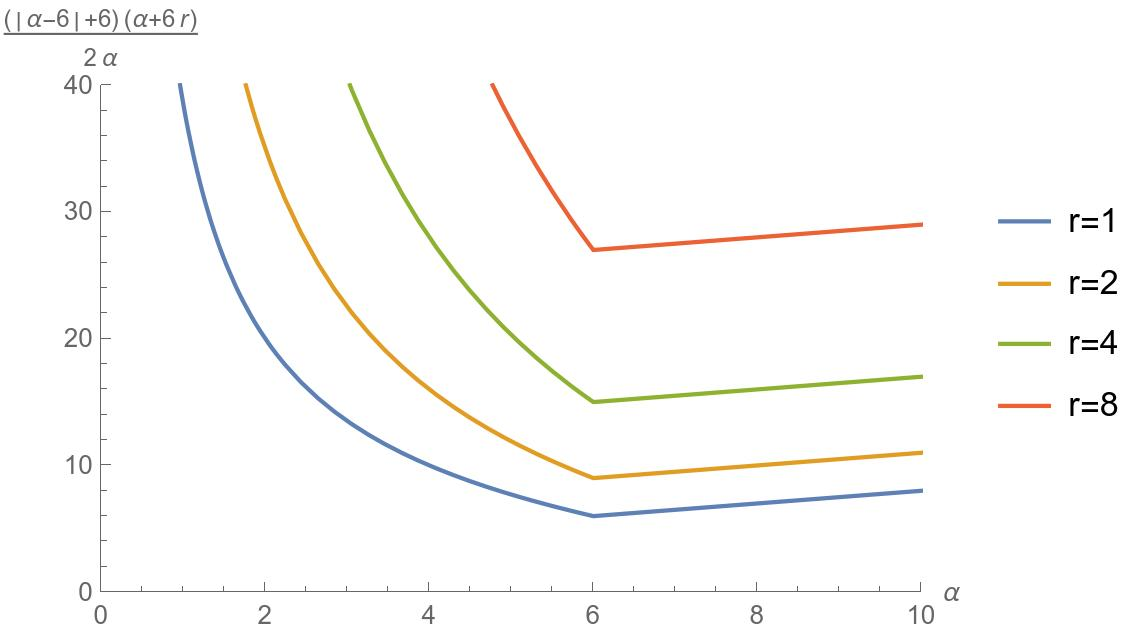
\includegraphics[scale =0.8]{optimal_alpha.jpeg}
    \caption{\footnotesize Plot of the bound obtained on $\Psi(\alpha)$ for different values of $r$. Visually it is clear that the minimum of this bound always occurs at $\alpha = 6$.}
    \label{optimal_alpha_fig}
\end{figure}

\section{Examples and Experiments}
\subsection{A Prototypical Use Case}
The prototypical application case for the HSS and IHSS iteration methods is the equilibrium state convection-diffusion equation. \cite{bai2003hermitian, bai2005block, bai2010newton, HUANG2014142} The convection-diffusion equation is in general given by (cite Thomas Stocker)

\begin{equation}
    \frac{\partial v}{\partial t} = \nabla \cdot (D \nabla v) - \nabla(v\vec{u})+ f,
\end{equation}
where $v$ is the unknown, $D$ is the diffusion coefficient, $\vec{u}$ is the velocity field of the medium, and $f$ is a source term. In the case of equilibrium flow, and assuming also that $D$ and $\vec{u}$ are constant, the convection-diffusion equation reduces to

\begin{equation}\label{prototypical_example}
    -\nabla^2 v + \vec{u}\cdot \nabla v = f.
\end{equation}

Equation \ref{prototypical_example} considered on the unit cube (or square) with Dirichlet boundary conditions serves as the main test for the HSS method. This is for two reasons. Firstly, it is time-independent: if there was a time-dependence, (and hence initial or final conditions) a brute force method of solving the PDE would simply involve a single term recurrence relation without a need for solving linear systems. [cite something] Moreover, unlike the Poisson equation (i.e. the case where $\vec{u} = 0$) which is Hermitian positive definite, the differential operator of the equilibrium state convection diffusion equation is non-Hermitian positive definite, hence it demonstrates more fully the advantages of the HSS method. Suppose we were to convert (\ref{prototypical_example}) into a linear set of equations by using a uniform step size $h = \frac{1}{N+1}$ in every dimension. We will denote the function $v$ evaluated at $(x_i = ih, y_j = jh, z_k = kh)$ by $v_{i,j,k}$, with $i,j,k = 0, 1, 2,\ldots, N+1$. The Dirichlet boundary conditoins impose the constraints $v_{0,j,k} = v_{i,0,k} = v_{i,j,0} = 0$ and also $v_{N+1,j,k} = v_{i,N+1,k} = v_{i,j,N+1} =0$. In our linearalisation, both the first and second derivatives are approximated by the central difference scheme, i.e.

\begin{align}
    \frac{\partial v}{\partial x}|_{(x_i, y_j, z_k)} &\approx \frac{v_{i+1,j,k} - v_{i-1,j,k}}{2h} \\
    \frac{\partial^2 v}{\partial x^2}|_{(x_i, y_j, z_k)} &\approx -\frac{2v_{i,j,k} - v_{i-1,j,k}-v_{i+1,j,k}}{h^2}
\end{align}
and similar in the $y$ and $z$ directions. Here we will introduce the following definitions.

\begin{definition} Let $X \in \bC^{m \times n}, \;  Y \in \bC^{p \times q}$. Then the Kronecker product of $X$ and $Y$, denoted $ X \otimes Y$, is the $(m \cdot p) \times(n \cdot q)$ matrix

    $$\begin{pmatrix}X_{11}Y && \ldots && X_{1n}Y \\
                    \vdots && &&\vdots \\
                    X_{m1}Y && \ldots && X_{mn}Y
                    \end{pmatrix} $$
\end{definition}

\begin{definition} Let $T$ be a $n \times m \times p$  two-tensor. Then $\vect(T)$ is the $nmk$ dimensional vector given by arranging  the elements $T$ through the first dimension, then through the second, and lastly through the third. In other words

    $$[\vect(T)]_{i + mj + kp}  = T_{i,j,k}$$
\end{definition}

For details about the Kronecker product and the $\vect(\cdot)$ function see \cite[][pp 274-276]{AppliedNumerical}. Let $\vec{u} = (u_x, u_y,u_z )$ and define the mesh Reynold's numbers

\begin{equation}
    r_x = \frac{u_x h}{2}, \; \; r_y = \frac{u_y h}{2}, \; \;  r_z = \frac{u_z h}{2}.
\end{equation}

Then, using the approximation scheme described, (\ref{prototypical_example}) can be written \cite{greif1999block, AppliedNumerical}

\begin{equation}
    A \cdot \vect(v) = h^2\vect(f),
\end{equation}

where

\begin{align}
    A = T_x \otimes I \otimes I + I \otimes T_y \otimes I + I \otimes I \otimes T_z,
\end{align}

with
\begin{equation}
    T_x = \tri(-1-r_x, 6, -1 + r_x), \; \; T_y = \tri(-1-r_y, 0 , -1+r_y), \; \; T_z = \tri(-1-r_z, 0, -1 + r_z).
\end{equation}
\subsection{Numerical Results}
    We implemented a numerical solver for the convection-diffusion equation in (\ref{prototypical_example}) using the IHSS iteration method. We used the source term

    \begin{equation}
        f(x,y,z) = S_0 \exp\left\{-\left((x-1/4)^2+(y-1/4)^2+(z-1/4)^2)\right)/r^2\right \}
    \end{equation}

    with $S_0 = 10$ and $r = 0.1$ and the initial guess $x^{(0)} = \vect(f)$. Additionally, in each trial iteration was terminated once the condition

    \begin{equation}
        \norm{Ax^{(k)} - b}_2 \leq 1.0 \times 10^{-5}
    \end{equation}

    was met. The GMRES method was used to resolve the inner systems in each iteration. We also took $u_\xi = u,  \; \xi \in \{ x ,y ,z \}$. To select a suitable value for $\alpha$, we compare the method proposed in \cite{HUANG2014142} (as discussed in Subsection 3.2) with the method we introduced in Subsection 3.3 and we share the results in Tables 2-4. where the system times, number of outer iterations and the average time per outer iteration are presented for some parameters. In each case the total number of grid points is $N^3$.

    We denote the estimate of optimal alpha obtained via our method by $\alpha_{\Psi} =6$, while that obtained via the method in \cite{HUANG2014142} is denoted by $\alpha_{\Phi}$. Table (something) shows the calculated values of $\alpha_{\Phi}$ for some different values of $u$. From this data it seems that $\alpha_{\Phi} \rightarrow 6 = \alpha_{\Psi}$ in the limit of large $u$. Moreoever, $\alpha_{\Psi}$ gives superior results for small $u$ as documented in Table \ref{calc_alpha_tilde}. These facts taken together seems to indicate that $\alpha_{\Psi}$ is indeed a better estimate than $\alpha_{\Phi}$ for $\alpha^\ast$ in the use case considered here.

    The Python code can be found in the \verb|HSS_exper.py| file. The \verb|test_HSS_exper.py| file tests the HSS and IHSS iteration implementation in \verb|HSS_exper.py|. The machine used was a personal computer with an Intel Core i7-8565 CPU and 16 GB of memory running Ubuntu 20.04.3. Options to record precise CPU times for a process are limited on the Python platform, so instead we elected to measure the average system time for each iteration. The product of this average time with the number of iterations then gives an estimate of the CPU time.

\begin{center}
    \begin{tabular}{|l | c | c|}
        \hline
        \multicolumn{2}{|c|}{$n=8$}\\
        \hline
        u & $\alpha_{\Phi}$ \\
        \hline
        1 & 0.00235 \\
        10 & 0.252 \\
        100 & 5.842 \\
        1000 & 5.998 \\
        10000 & 5.99998 \\
        \hline
    \end{tabular}
\captionof{table}{}{\label{calc_alpha_tilde}}
\end{center}

\begin{center}
\begin{tabular}{|l | c | c|}
    \hline
    \multicolumn{3}{|c|}{$N = 8$, $u = 1$}\\
    \hline
     & $\alpha_{\Phi} = 0.00235$ & $ \alpha_{\Psi}$  \\
     \hline
    Outer iterations & 500+\footnote{The algorithm did not converge after 500 iterations in this case} & 118 \\
    Average time per iteration (ms) & 302 & 279 \\
    Estimated CPU time(s) & - & 32.9 \\
    \hline
\end{tabular}
\captionof{table}{}{\label{}}
\end{center}

\begin{center}
\begin{tabular}{|l | c | c|}
    \hline
    \multicolumn{3}{|c|}{$N = 8$, $u = 10$}\\
    \hline
     & $\alpha_{\Phi} = 0.252$ & $ \alpha_{\Psi}$  \\
     \hline
    Outer iterations & 191 & 40 \\
    Average time per iteration (ms) & 2501 & 465 \\
    Estimated CPU time(s) & 477.6 & 18.6 \\
    \hline
\end{tabular}
\captionof{table}{}{\label{}}
\end{center}

\begin{center}
\begin{tabular}{|l | c | c|}
    \hline
    \multicolumn{3}{|c|}{$N = 8$, $u = 1000$}\\
    \hline
     & $\alpha_{\Phi} = 5.998$ & $ \alpha_{\Psi}$  \\
     \hline
    Outer iterations & 80 & 80 \\
    Average time per iteration (ms) & 2186 & 2536 \\
    Estimated CPU time(s) & 174.8 & 202.8 \\
    \hline
\end{tabular}
\captionof{table}{}{\label{}}
\end{center}




\subsection{Discussion}
Given that $A$ fulfils the assumptions outlined in (\ref{herm}) and (\ref{skew_herm}), the method proposed by us for the selection of $\alpha$ outperforms that proposed in \cite{HUANG2014142}. Moreover, $\alpha_{\Phi} \rightarrow \alpha_{\Psi}$ in the limit of large $u$, and the performace of the two methods converges. This new method is also more suitable for matrix-free implementations since no explicit information about $A$, $H$, or $S$ is needed to compute $\alpha_{\Psi} =6$ (other than their sparsity structure which is assumed). However, this new method is far more limited in its use cases as it makes very strong assumption about the structure of $H$ and $S$.



\printbibliography



\begin{figure}[h]
    \centering
    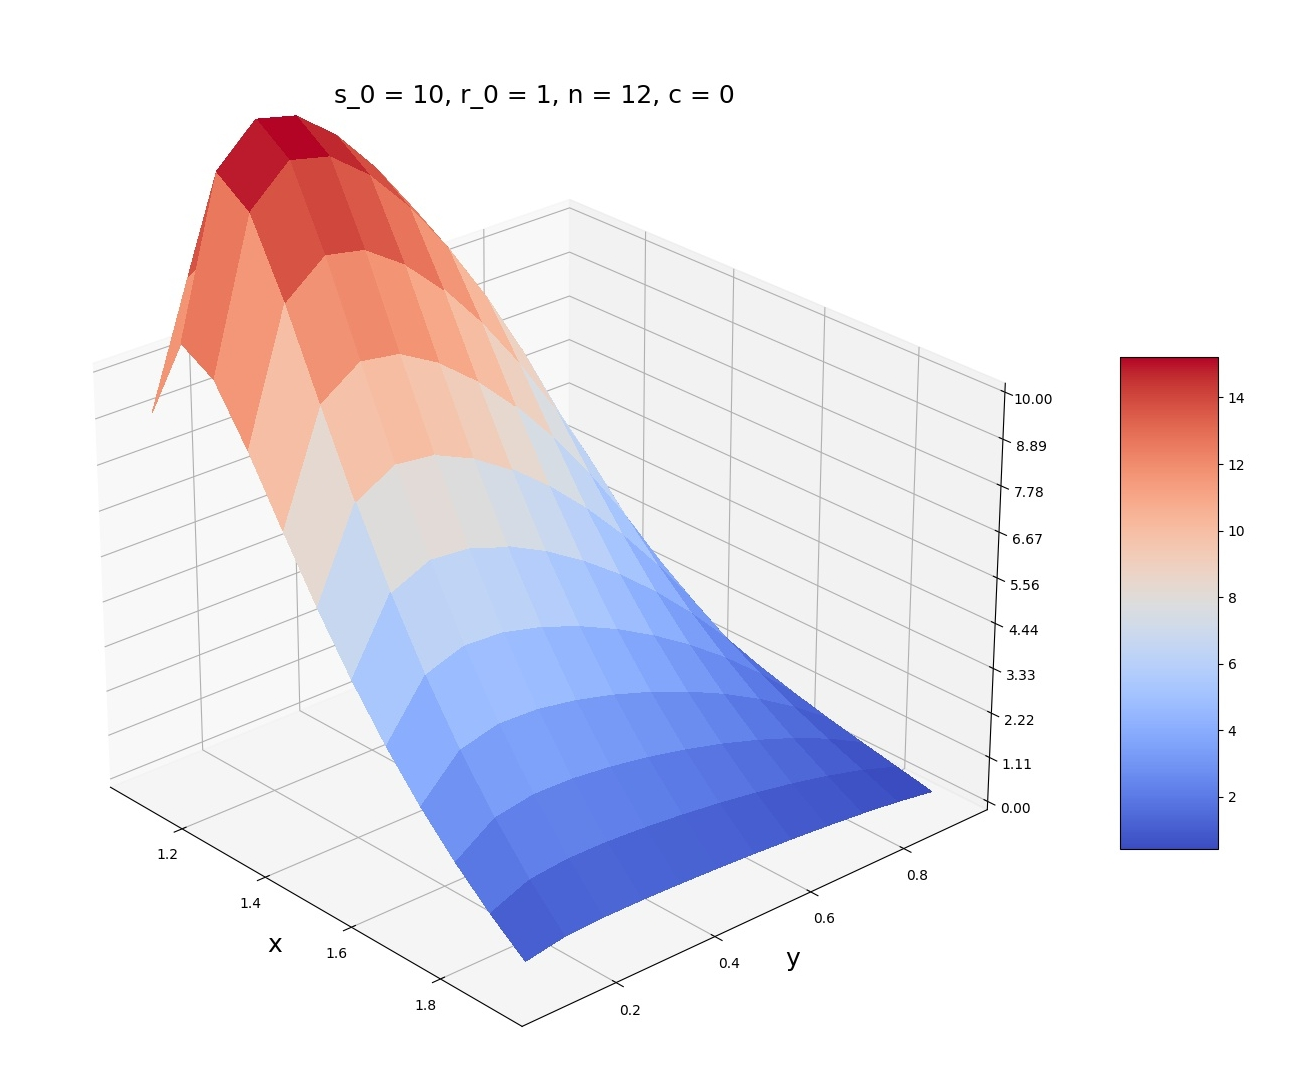
\includegraphics[scale = 0.3]{./graphics/typical_solution.jpeg}
    \caption{A typical solution obtained using our solver. Included for no particular reason.}
    \label{typical_graph}
\end{figure}

\end{document}
